\section{Buck-, Boost- und Buck-Boost-Converter}

DC-DC-Wandler sind spezielle Gleichstromsteller mit Energiespeicher.
Diese Section gibt ein einheitliches Vorgehen zur Analyse von Buck-, Boost- und Buck-Boost-Wandlern
im kontinuierlichen Strombetrieb (CCM), mit und ohne Ausgangskondensator.

\smallskip
\paragraph{Zentrale Zustände und Annahmen}

Zustandsgrössen:
\[
x(t) = \begin{bmatrix} i_L(t) \\ u_C(t) \end{bmatrix}
\]

Kontinuität:
\[
i_L(t^-) = i_L(t^+), 
\qquad 
u_C(t^-) = u_C(t^+)
\]

Grundbilanz im stationären Betrieb:
\[
\cbl{\overline{u_L} = 0}
\qquad\text{(Voltsekunden-Bilanz)}
\]
\[
\cbl{\overline{i_C} = 0}
\qquad\Rightarrow\qquad
\overline{i_L} = \overline{i_o}
\]

Zeitkonstante des R--L-Zweigs:
\[
\tau = \frac{L}{R}
\]

\smallskip
\paragraph{Grenzinduktivität für kontinuierlichen Betrieb}
\[
L_{\min} = \frac{(1-d)R}{2 f_s}
\]

\textbf{Zielbild:}
\begin{itemize}
    \item Topologie sicher identifizieren
    \item EIN- und AUS-Gleichungen angeben
    \item Mittelwert mit Voltsekunden-Bilanz bestimmen
    \item Ripple mit $L$ und $C$ berechnen
\end{itemize}

% -------------------------------------------------
\subsection{Allgemeines Schaltintervall-Schema}

Für jedes Schaltintervall mit konstanter Topologie gilt:

\[
A x + B u = 0
\quad \Rightarrow \quad
\dot{x} = f(x,u)
\]

Vorgehen:

\begin{enumerate}
 \item Topologie festlegen (EIN oder AUS).
 \item DGL für dieses Intervall aufstellen.
 \item Lösung:
 \[
 x(t) = x_\infty + (x(t_0)-x_\infty)e^{-(t-t_0)/\tau}
 \]
 \item Endwert als Anfangsbedingung des nächsten Intervalls verwenden.
\end{enumerate}

Stationärer Betrieb:
\[
x(0) = x(T_s)
\]

\subsection{Allgemeines Grundprinzip}

Alle DC-DC-Wandler arbeiten mit:

\begin{itemize}
    \item Schalter
    \item Diode (oder synchroner Schalter)
    \item Induktivität $L$
    \item Glättkondensator $C$
\end{itemize}

Grundgleichung:
\[
\cbl{u_L = L \frac{di_L}{dt}}
\qquad\Rightarrow\qquad
\cbl{\overline{u_L} = 0}
\]

Kondensatorstrom:
\[
i_C(t) = i_L(t) - i_o
\qquad\Rightarrow\qquad
\overline{i_C} = 0
\]

\crd{\textrightarrow\ Diese zwei Bilanzen sind der Startpunkt jeder Aufgabe.}

% -------------------------------------------------
\subsection{Allgemeines Schaltintervall-Schema}

Für jedes Schaltintervall mit konstanter Topologie gilt:

\[
A x + B u = 0
\quad \Rightarrow \quad
\dot{x} = f(x,u)
\]

Vorgehen:

\begin{enumerate}
 \item Topologie festlegen (EIN oder AUS).
 \item DGL für dieses Intervall aufstellen.
 \item Lösung:
 \[
 x(t) = x_\infty + (x(t_0)-x_\infty)e^{-(t-t_0)/\tau}
 \]
 \item Endwert als Anfangsbedingung des nächsten Intervalls verwenden.
\end{enumerate}

Stationärer Betrieb:
\[
x(0) = x(T_s)
\]

\subsection{Buck-Converter (Abwärtssteller)}

\begin{center}
    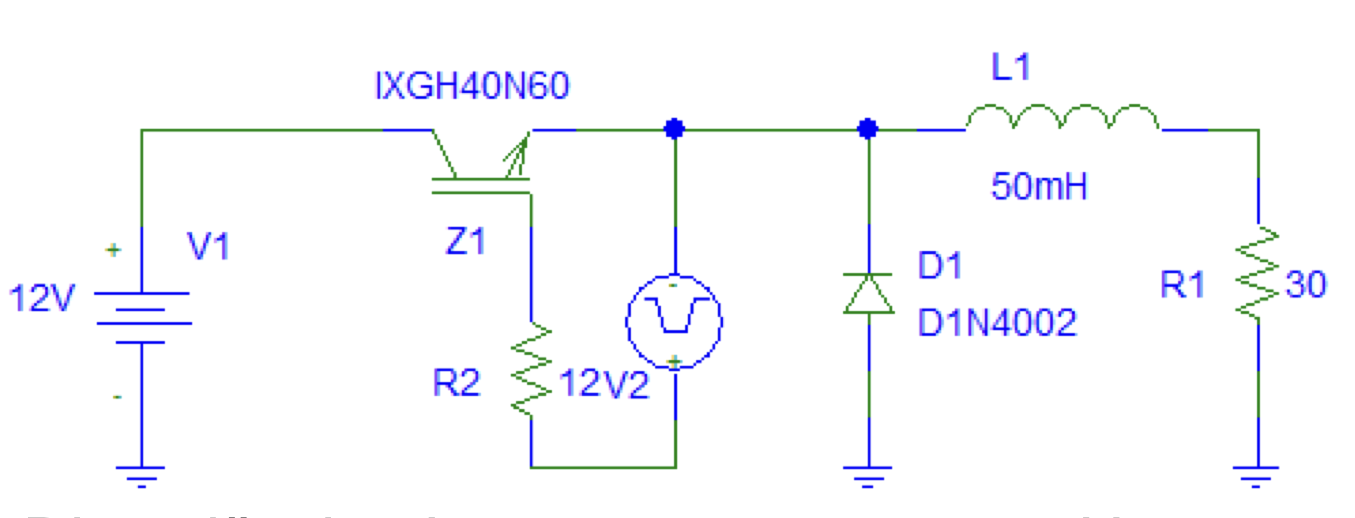
\includegraphics[width=0.85\linewidth]{images/Buckconverter.png}
\end{center}

Zeitverlauf Buck-Converter:
\begin{center}
    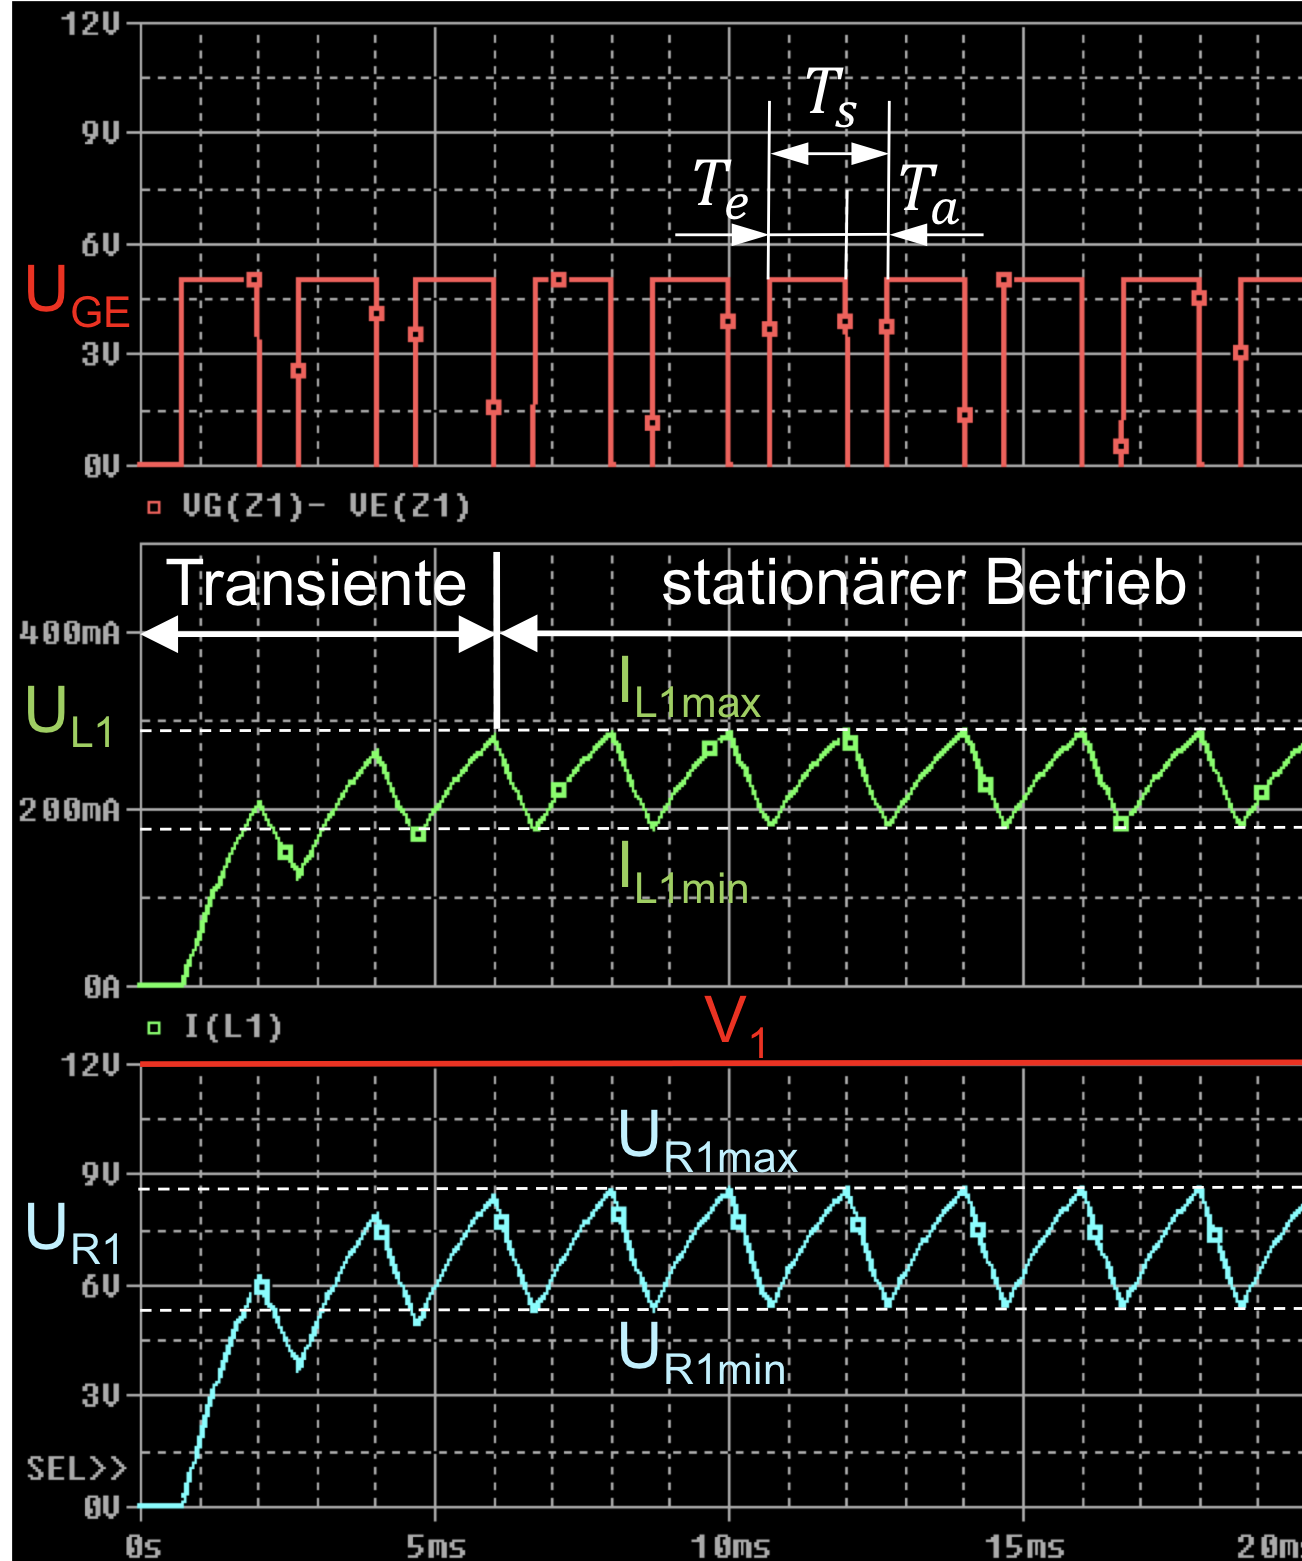
\includegraphics[width=0.85\linewidth]{images/Buckconverter_verlauf.png}
\end{center}

Ziel:
\[
u_2 < U_{DC}
\]

\paragraph{Voltsekunden-Bilanz}
\[
(U_{DC}-u_2)\, dT_s + (-u_2)(1-d)T_s = 0
\qquad\Rightarrow\qquad
\cbl{u_2 = d\,U_{DC}}
\]

\paragraph{EIN- und AUS-Gleichungen}

EIN-Phase:
\[
u_L = U_{DC} - u_2,
\qquad
i_C = i_L - i_o
\]

AUS-Phase:
\[
u_L = -u_2,
\qquad
i_C = i_L - i_o
\]

\paragraph{Strom- und Spannungsripple}

\[
\Delta i_L = \frac{(U_{DC}-u_2)}{L} \, d T_s
\]

\[
\Delta u_2 \approx \frac{\Delta i_L}{8 f_s C}
\]

Eigenschaften:
\begin{itemize}
    \item Ausgangsspannung kleiner als Eingang
    \item Kontinuierlicher Ausgangsstrom
\end{itemize}

% -------------------------------------------------
\subsection{Boost-Converter (Aufwärtssteller)}

\begin{center}
    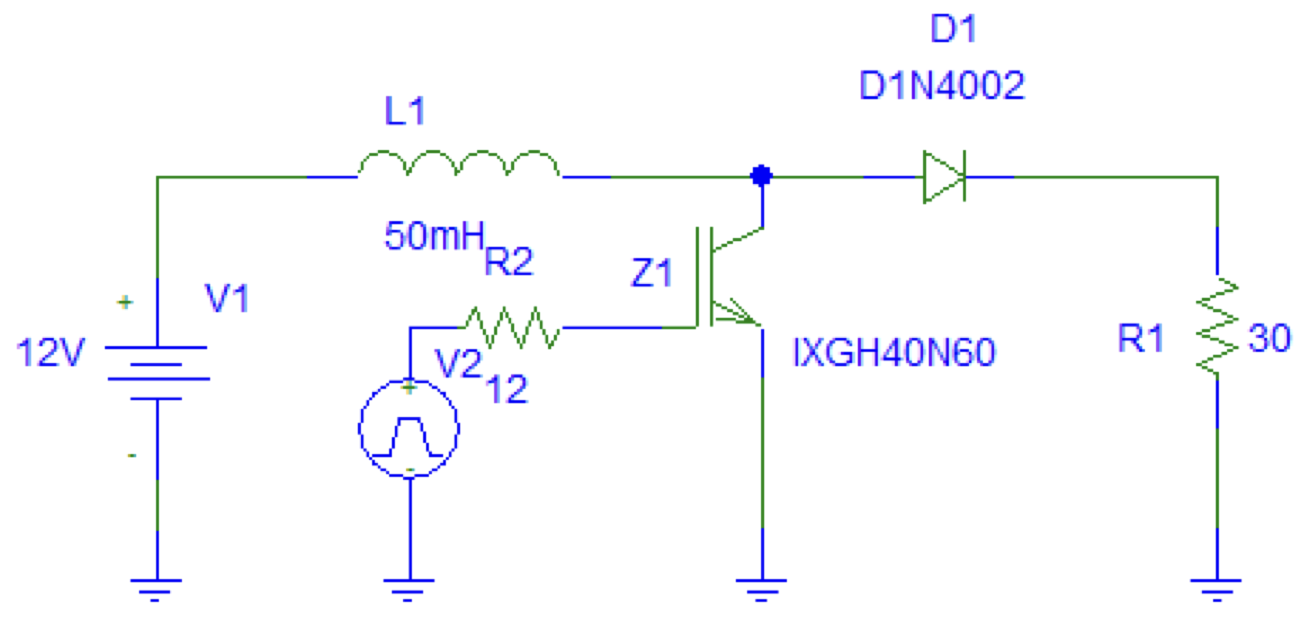
\includegraphics[width=0.85\linewidth]{images/Boostconv.png}
\end{center}

Zeitverlauf Boost-Converter:
\begin{center}
    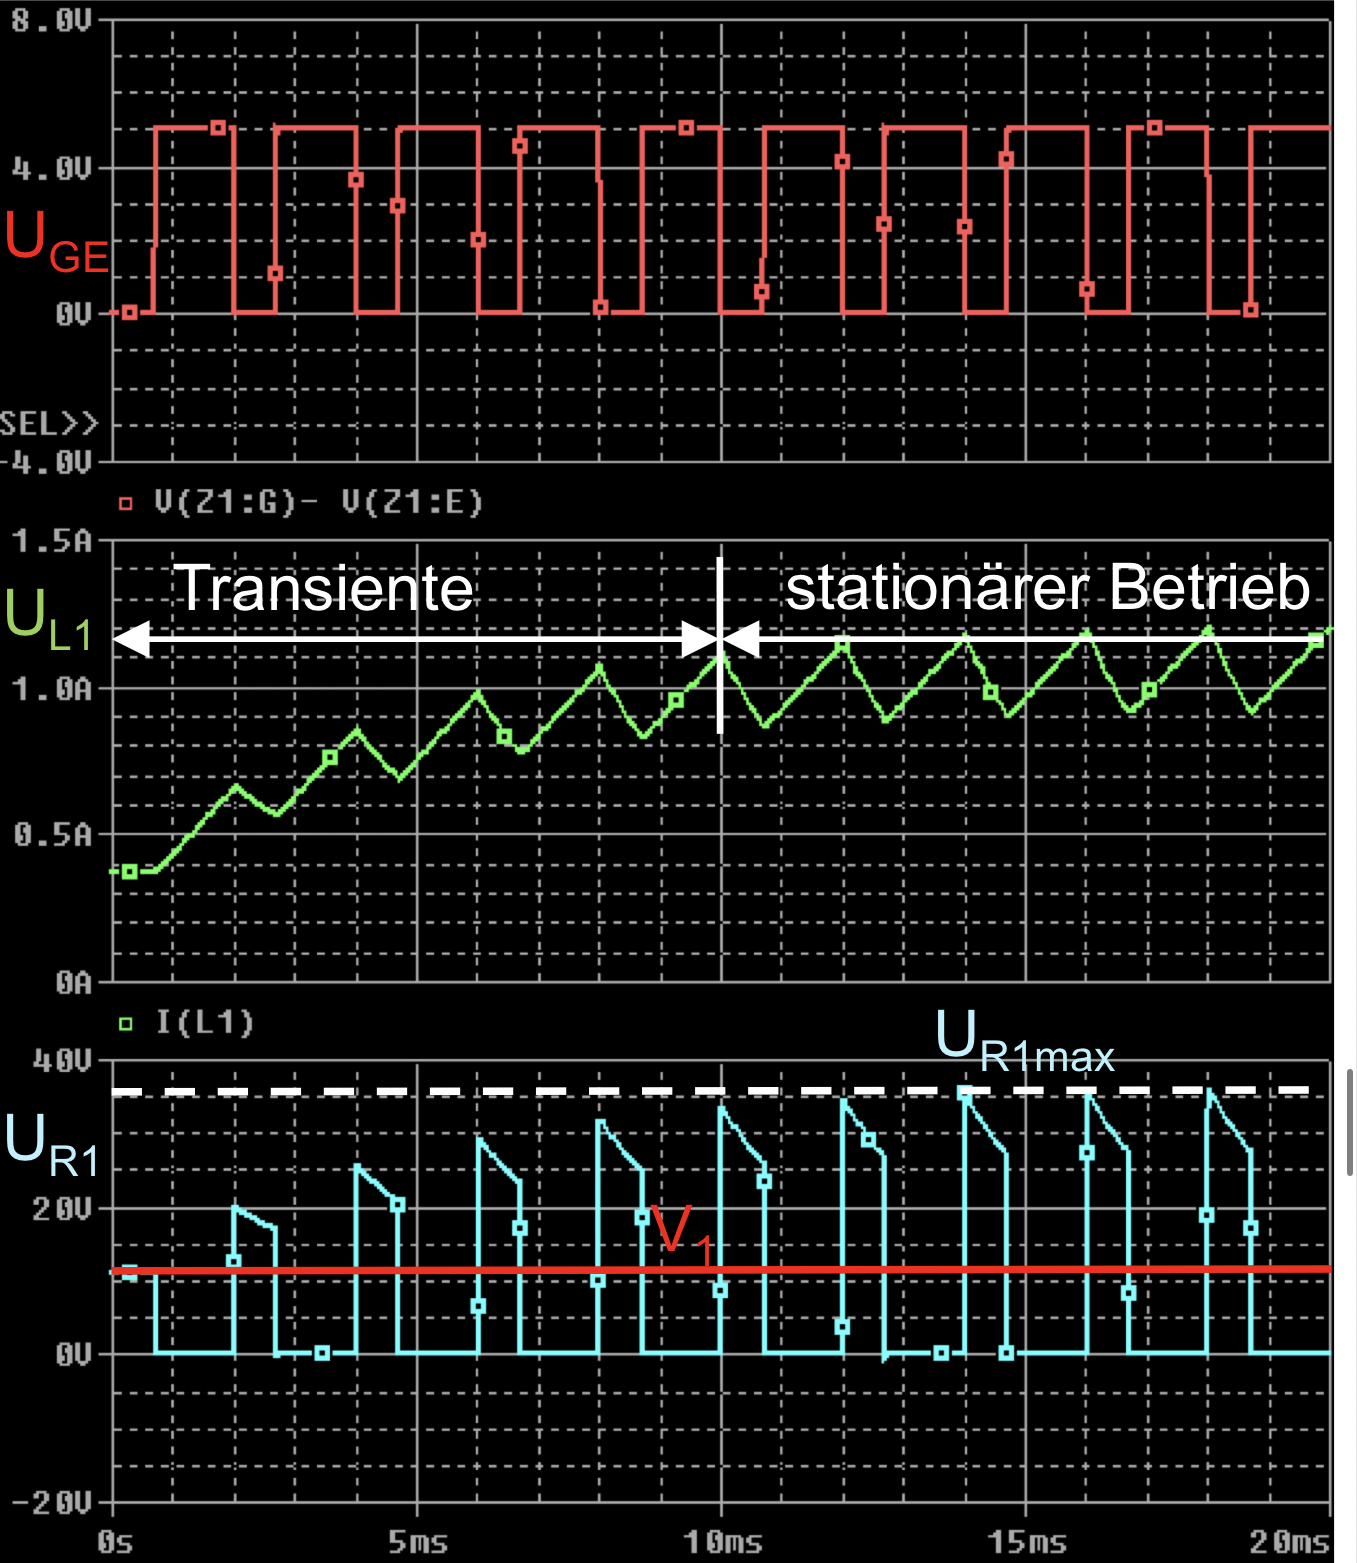
\includegraphics[width=0.85\linewidth]{images/Boostconv_verlauf.png}
\end{center}

Ziel:
\[
u_2 > U_{DC}
\]

\paragraph{Voltsekunden-Bilanz}
\[
U_{DC}\, dT_s + (U_{DC}-u_2)(1-d)T_s = 0
\qquad\Rightarrow\qquad
\cbl{u_2 = \frac{U_{DC}}{1-d}}
\]

\paragraph{EIN- und AUS-Gleichungen}

EIN-Phase (Diode sperrt):
\[
u_L = U_{DC},
\qquad
i_C = - i_o
\]

AUS-Phase (Diode leitet):
\[
u_L = U_{DC} - u_2,
\qquad
i_C = i_L - i_o
\]

\paragraph{Ripple-Näherungen}

\[
\Delta i_L = \frac{U_{DC}}{L} \, d T_s
\]

\[
\Delta u_2 \approx \frac{i_o}{C} (1-d) T_s
\]

Eigenschaften:
\begin{itemize}
    \item Ausgangsspannung grösser als Eingang
    \item Eingangsstrom gepulst
\end{itemize}

% -------------------------------------------------
\subsection{Buck-Boost-Converter}

\begin{center}
    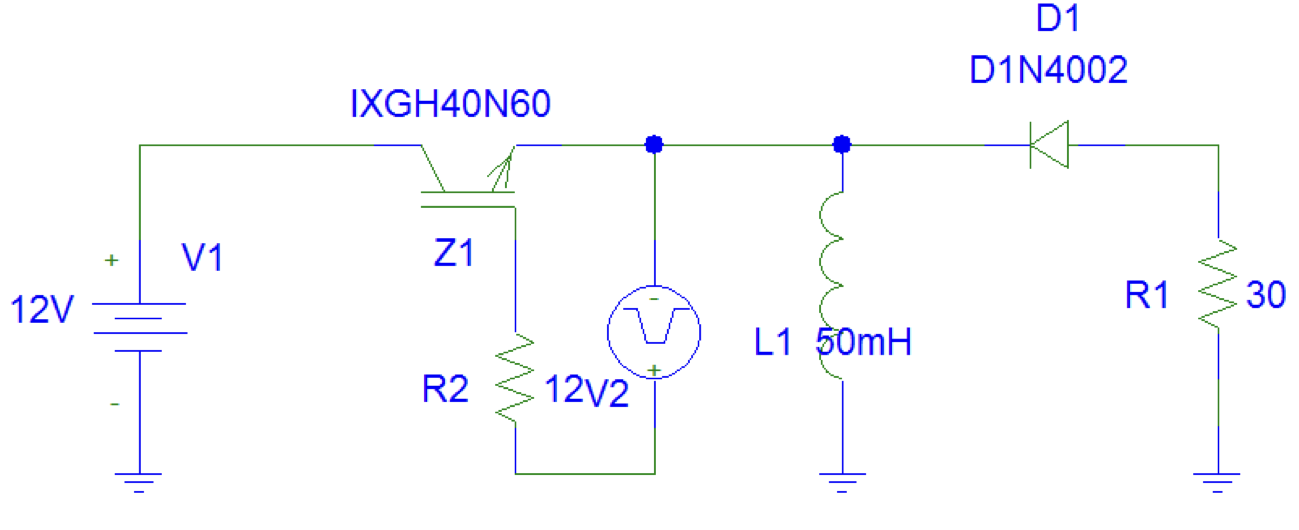
\includegraphics[width=0.85\linewidth]{images/Buckboostconv.png}
\end{center}

Zeitverlauf Buck-Boost-Converter:
\begin{center}
    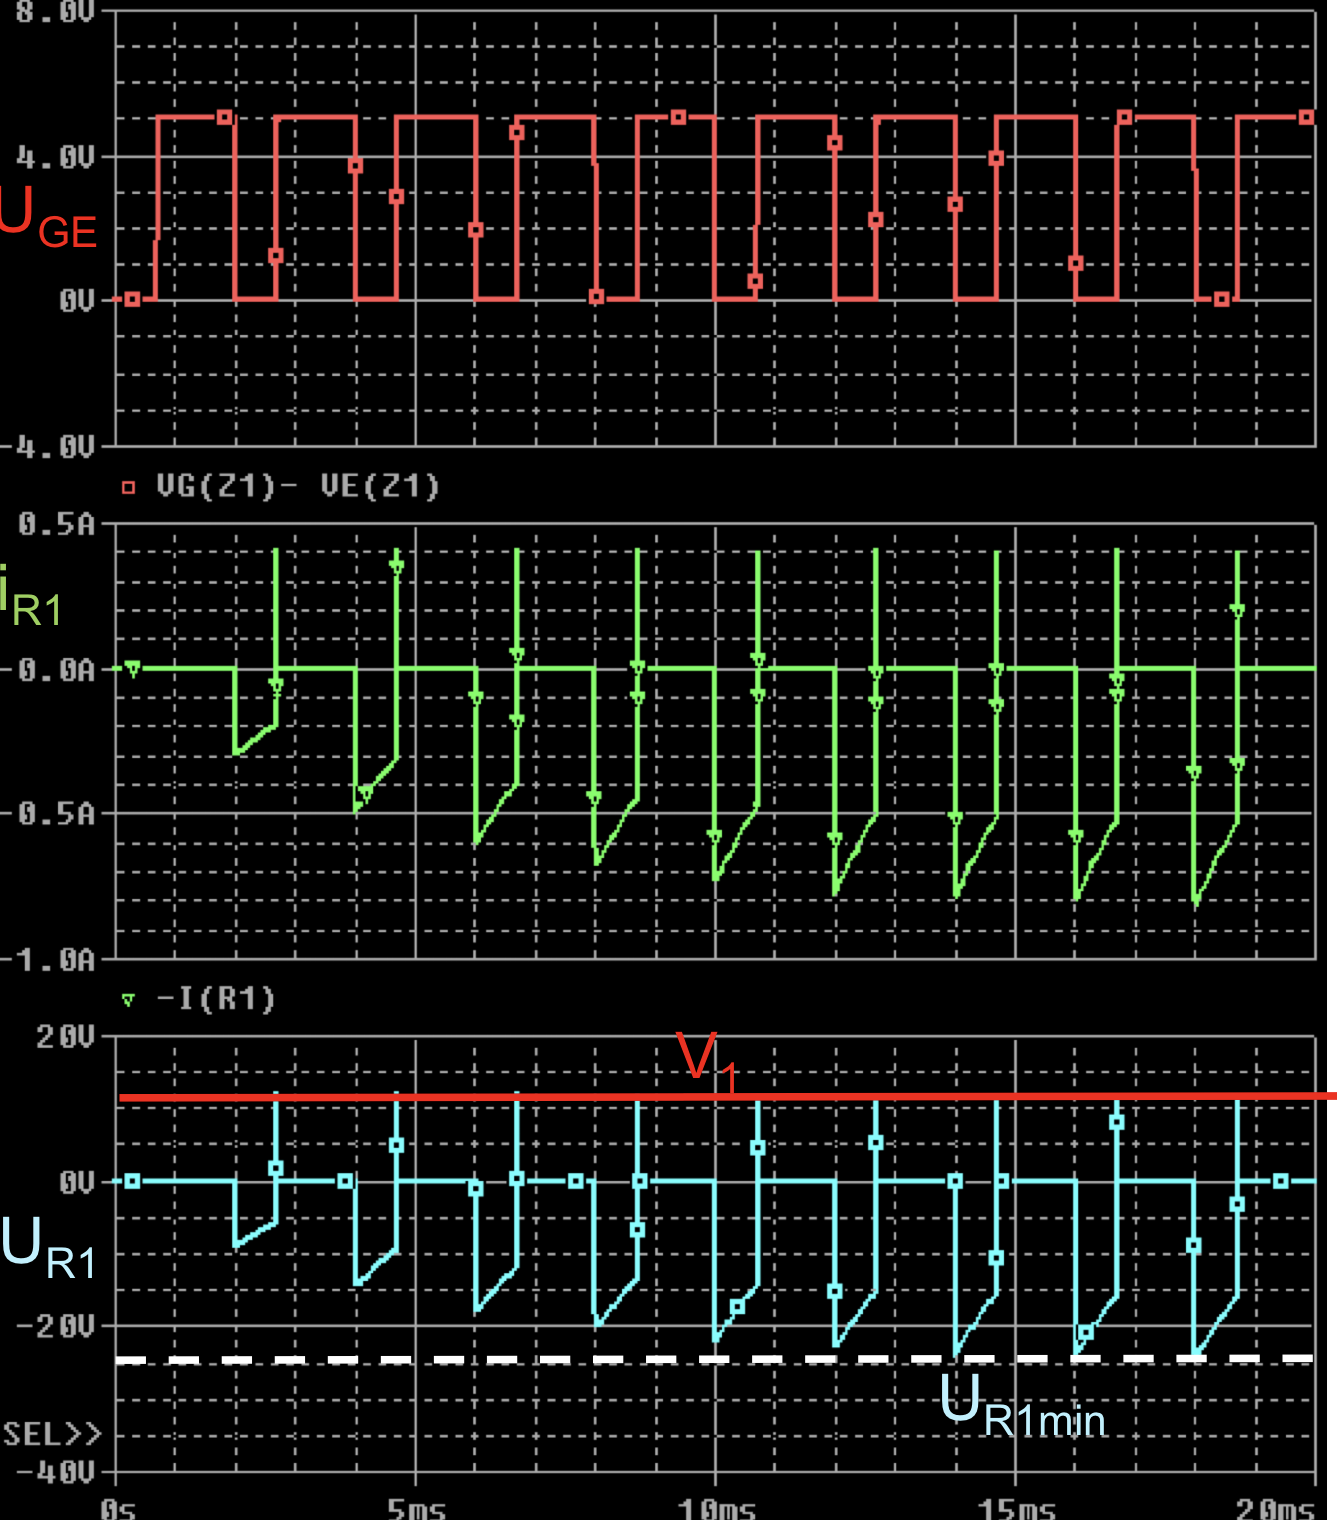
\includegraphics[width=0.85\linewidth]{images/Buckboostconv_verlauf.png}
\end{center}

Ziel:
\[
u_2 < 0 \quad \text{oder} \quad |u_2| > U_{DC}
\]

\paragraph{Voltsekunden-Bilanz}
\[
U_{DC}\, dT_s + (-u_2)(1-d)T_s = 0
\qquad\Rightarrow\qquad
\cbl{u_2 = -\frac{d}{1-d} U_{DC}}
\]

\paragraph{EIN- und AUS-Gleichungen}

EIN-Phase:
\[
u_L = U_{DC},
\qquad
i_C = - i_o
\]

AUS-Phase:
\[
u_L = -u_2,
\qquad
i_C = i_L - i_o
\]

\paragraph{Ripple-Näherungen}

\[
\Delta i_L = \frac{U_{DC}}{L} \, d T_s
\]

\[
\Delta u_2 \approx \frac{i_o}{C} (1-d) T_s
\]

Eigenschaften:
\begin{itemize}
    \item Polaritätsumkehr
    \item Spannung grösser oder kleiner als Eingang möglich
\end{itemize}

% -------------------------------------------------
\subsection{Vergleich der DC-DC-Wandler}

\begin{center}
\begin{tabular}{l|c|c|c}
 & Buck & Boost & Buck-Boost \\ \hline
$u_2/U_{DC}$ & $d$ & $\frac{1}{1-d}$ & $-\frac{d}{1-d}$ \\
Polarität & gleich & gleich & \cbl{invertiert} \\
$u_2<U_{DC}$ & \cbl{ja} & nein & ja \\
$u_2>U_{DC}$ & nein & \cbl{ja} & ja \\
\end{tabular}
\end{center}

% -------------------------------------------------
\subsection{Allgemeines Lösungsschema für Prüfungsaufgaben}

\begin{enumerate}
    \item Topologie identifizieren (Buck, Boost, Buck-Boost).
    \item Betriebsart prüfen: CCM oder DCM.
    \item EIN- und AUS-Gleichungen für $u_L$ und $i_C$ angeben.
    \item Voltsekunden-Bilanz $\overline{u_L}=0$ anwenden.
    \item Stromripple $\Delta i_L$ berechnen.
    \item Spannungsripple $\Delta u_2$ aus $C$ bestimmen.
    \item Falls Zeitbereich gefragt: Exponential- oder lineare Lösungen anwenden.
\end{enumerate}

\subsection{Abgrenzung zu klassischen Gleichstromstellern}

\begin{itemize}
    \item Klassischer Gleichstromsteller: direkte Pulsweitensteuerung der Last.
    \item DC-DC-Wandler: Energieübertragung über Induktivität mit Spannungsanpassung.
\end{itemize}

\crd{\textrightarrow\ Buck/Boost/Buck-Boost sind Gleichstromsteller mit Energiespeicher.}
